\chapter{Dynamical equations rescaling}

Starting from the standard Generalized Lotka-Volterra (GLV) equations, which govern the dynamics of interacting nodes in our network:
$$\dot{x}_i = x_i \left( 1 - x_i + \sum_j W_{ij} x_j \right)$$
we encounter severe computational divergences as the interaction strength $\mu$ approaches and exceeds the critical threshold $\mu_c$. To study the system across this critical regime without triggering numerical overflow, we perform a coordinate transformation that maps the unbounded trajectories onto a bounded probability space.

\section{Mapping to the Probability Simplex and Time Rescaling}

We introduce a macroscopic scaling factor $M(t)$ representing the total system abundance, and map the absolute abundances $x_i(t)$ to relative fractions $y_i(t)$:
$$\begin{cases}
M(t) = \sum_j x_j(t) \\
y_i(t) = \frac{x_i(t)}{M(t)}
\end{cases}$$
By definition, the rescaled variables are bounded on the probability simplex such that $y_i(t) \ge 0 \quad \forall t$ and $\sum_j y_j(t) = 1$.

While this transformation bounds the variables $y_i$, the resulting dynamical equations still depend multiplicatively on the macroscopic envelope $M(t)$, which diverges for $\mu > \mu_c$. To stabilize the integration, we introduce a non-linear stretching of time by defining a new time variable $\tau$:
$$\frac{d\tau}{dt} = M(t)$$
Applying this change of variables and time rescaling to the original GLV system (the full step-by-step algebraic derivation is provided in Appendix A), we obtain the following stable, bounded set of dynamical equations:
$$\frac{dy_i}{d\tau} = y_i \left[ \sum_{j=1}^N W_{ij} y_j - y^T W y - y_i + y^T y \right]$$
$$\frac{dM}{d\tau} = 1 + M \left[ y^T W y - y^T y \right]$$
$$\frac{dt}{d\tau} = \frac{1}{M}$$
We can also express the dynamics of the simplex directly in a fully vectorized form, utilizing element-wise multiplication ($\odot$) and a vector of ones ($\mathbf{1}$):
$$\frac{dy}{d\tau} = y \odot \left[ Wy - (y^T W y)\mathbf{1} - y + (y^T y)\mathbf{1} \right]$$
Crucially, the evolution of the relative fractions $y(\tau)$ is now completely decoupled from the divergent macroscopic envelope $M$. However, we concurrently integrate $M(\tau)$ and $t(\tau)$ alongside $y(\tau)$ to allow for the exact reconstruction of the unscaled physical trajectories $x(t)$ whenever necessary.

\section{Theoretical Limitations and the Need for Numerical Integration}

While closed-form analytical solutions for the equilibrium state $(M^*, y^*)$ can be derived mathematically (see Appendix B), they are valid only under strictly cooperative assumptions ($\mu < \mu_c$) where an interior fixed point exists and all species survive.

However, as the interaction strength reaches and exceeds the critical threshold ($\mu \ge \mu_c$), the theoretical mean-field behavior predicts the onset of relative extinctions. In this divergent regime, hub nodes grow exponentially faster than the rest of the network, forcing the relative fractions of lower-degree nodes toward zero. Consequently, the full $N \times N$ matrix $(I-W)$ is no longer invertible, and the true equilibrium transitions into a Linear Complementarity Problem (LCP) restricted to surviving active nodes.

Because this analytical framework breaks down precisely at the critical topological boundary we aim to study, we abandon the search for closed-form static equilibria. Instead, our methodology relies entirely on the numerical integration of the exact, bounded dynamical equations derived above to capture the critical transient fluctuations of the system.

\section{Numerical Integration}

The function that will be fed into the solver is the following:

\noindent
\begin{minipage}{\textwidth}
\begin{minted}{python}
def rescaled_glv_sparse(tau, state, N, W_sparse):
    """
    The numerically stable, rescaled ODE system.
    state = [y_1, y_2, ..., y_N, M, t]
    """
    y = state[:N]
    M = state[N]
    # t = state[N+1] is tracked by the solver, but doesn't affect the derivatives

    # fast sparse matrix multiplication
    F = W_sparse @ y

    # vectorized scalars
    phi = np.dot(y, F)     # The average network fitness: y^T W y
    sq_sum = np.sum(y**2)  # The self-competition penalty: y^T y

    # differential equations
    dydtau = y * (F - phi - y + sq_sum)
    dMdtau = 1.0 + M * (phi - sq_sum)
    dtdtau = 1.0 / M

    return np.concatenate((dydtau, [dMdtau], [dtdtau]))
\end{minted}
\end{minipage}

\vspace{10pt}
The only thing we must careful about is to set a max step of about $10^3$ otherwise the trajectories will reach a plateau but a big max step could introduce noise that would then destroy the unscaled trajectory.

\section{M(t) Scaling ($\sigma = 0$, $0<\mu<\mu_c$)}

In true time the evolution of $M(t)$ is governed by:
\begin{equation}
    \frac{dM}{dt} = M - M^2(y^Ty - y^T Wy)
\end{equation}

\subsection{$\mu < \mu_c$}

Effectively $(I - W)$ is positive definite, hence the growth is logistic with a dynamic carry capacity and $M^* = 0$ or $M^* = \left[(y^*)^T(I-W)y^*\right]^{-1} = 1/c$

Now onto the solution for $y^*$ (solution for $y^*=0$ is inadmissible since $\sum_j y_j = 1$):
\begin{equation}
    \begin{aligned}
    0 &= -(I - W)y^* + c\mathbf{1} \\
    y^* &= c (I - W)^{-1} \mathbf{1}
    \end{aligned}
\end{equation}
we can now use the normalization condition $\mathbf{1}^T y^* = 1$
\begin{equation}
\begin{aligned}
        \mathbf{1}^T y^* = c \Big( \mathbf{1}^T (I - W)^{-1} \mathbf{1} \Big) \\
        1 = c \Big( \mathbf{1}^T (I - W)^{-1} \mathbf{1} \Big)
\end{aligned}
\end{equation}
hence:
\begin{equation}
    c = \frac{1}{\mathbf{1}^T (I - W)^{-1} \mathbf{1}}
\end{equation}
then
\begin{equation}
   y^* = \frac{(I - W)^{-1} \mathbf{1}}{\mathbf{1}^T (I - W)^{-1} \mathbf{1}}
\end{equation}
finally
\begin{equation}
    M^* = \frac{1}{c} = \mathbf{1}^T (I - W)^{-1} \mathbf{1}
\end{equation}

\section{Plots}

Here are the results of the integration of the rescaled variables compared with the unscaled trajectories, a sample of 100 trajectories is shown. For all the plots the exponential degree distribution has been chosen.

% FIXME: figure file pending — uncomment once rescaled_unscaled_mu_minus_2.png lands in figures/
% \begin{figure}[htbp]
%     \centering
%     \begin{minipage}{1\linewidth}
%         \centering
%         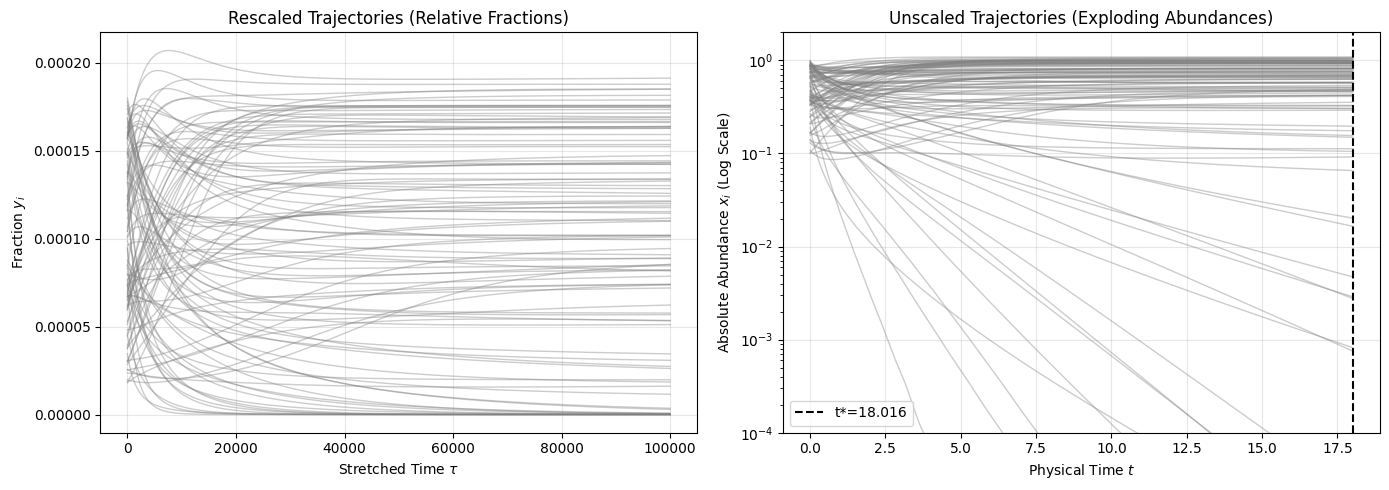
\includegraphics[width=\linewidth]{rescaled_unscaled_mu_minus_2.png}
%         \caption{$N=10^4$, $C=50$, $\mu = -2 < \mu_c \approx 0.5458$, $\sigma=0.5$}
%         \label{fig:stable-unscaled}
%     \end{minipage}
%
%     \vspace{1.5em}
%
%     \begin{minipage}{1\linewidth}
%         \centering
%         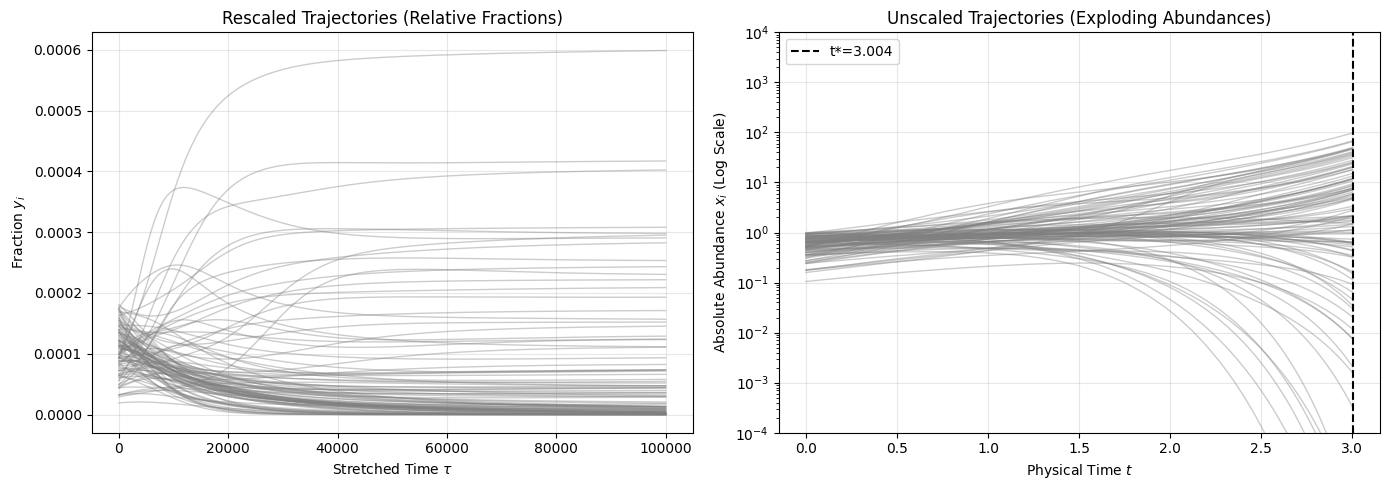
\includegraphics[width=\linewidth]{rescaled_unscaled_mu_05.png}
%         \caption{$N=10^4$, $C=50$, $\mu = 0.5 \approx \mu_c \approx 0.5458$, $\sigma=0.5$}
%         \label{fig:divergin-unscaled}
%     \end{minipage}
% \end{figure}

\section{Finding $\mu_c$}

The theoretical result for $\mu_c$ fails in the context of finite graphs, hence we must find a new way to calculate the critical value for $\mu$. Here is where the rescaled equations play their fundamental role since they are blind to the crossing of $\mu_c$ we can integrate the rescaled equations for different values of $\mu$ inputting the same max rescaled time, then converting back to true time we can clearly see where the $\mu_c$ actually happened.

% FIXME: figure file pending — uncomment once true_mu_c.png lands in figures/
% \begin{figure}[h]
%     \centering
%     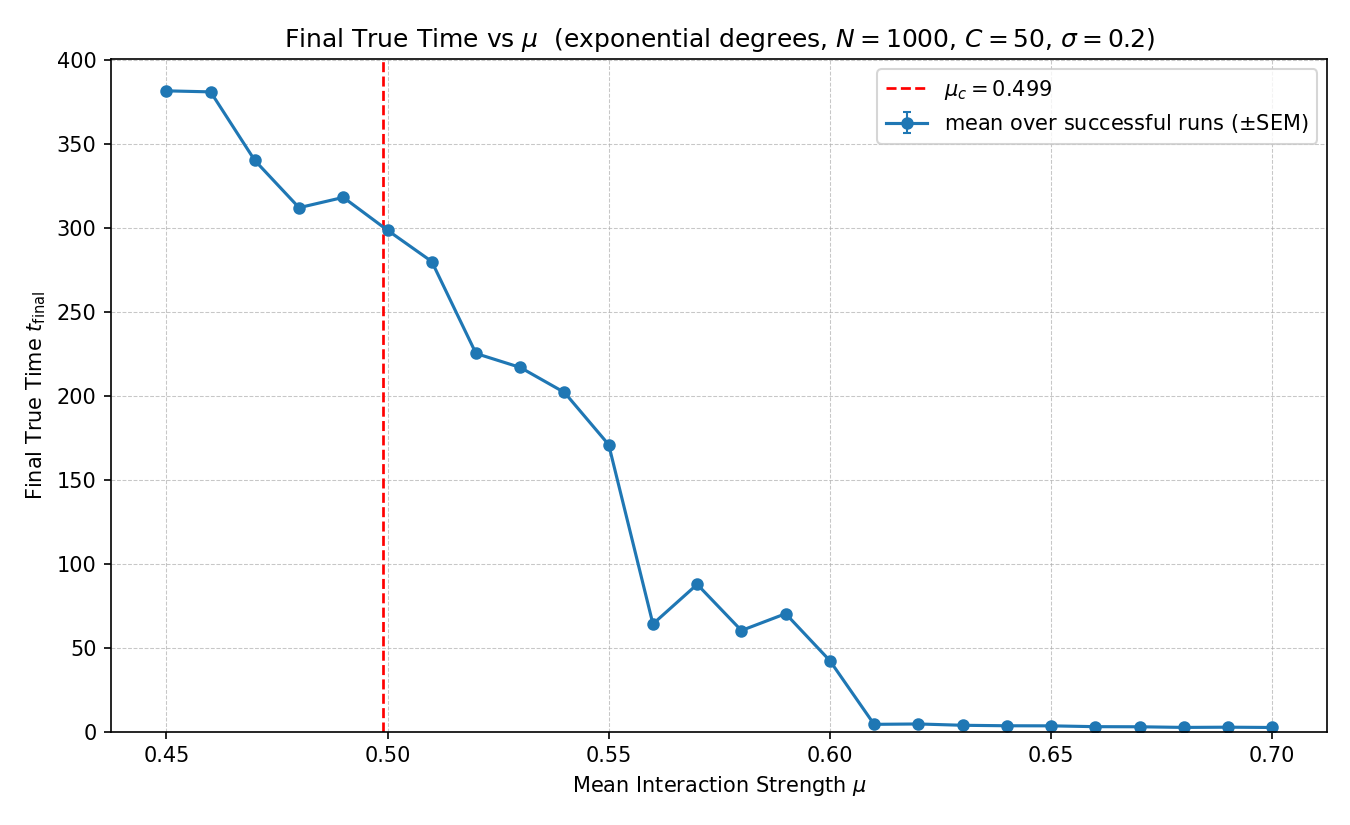
\includegraphics[width=1\linewidth]{true_mu_c.png}
%     \caption{Enter Caption}
%     \label{fig:placeholder-true-mu-c}
% \end{figure}

This method is very robust because true time is an integrated quantity of the inverse of $M(\tau)$.

We can characterize the distance of the actual value for $\mu_c$ over different realizations of the system looking at the distribution of the distance between the empirical and the theoretical one yielding this histogram. Histogram has been built on 100 different graph realizations due to constraints in computation time.

% FIXME: figure file pending — uncomment once theoretical-vs-actual.png lands in figures/
% \begin{figure}[h]
%     \centering
%     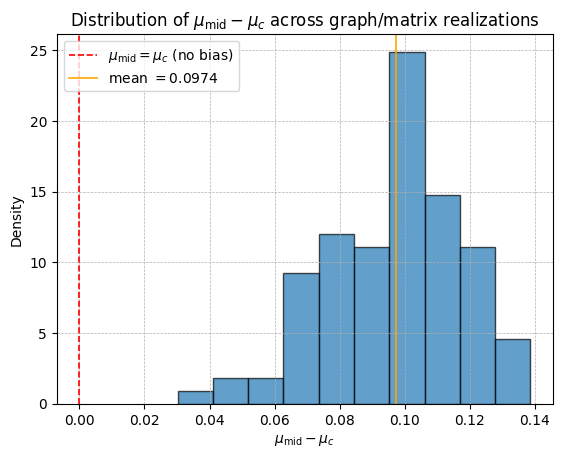
\includegraphics[width=0.75\linewidth]{theoretical-vs-actual.png}
%     \caption{Enter Caption}
%     \label{fig:placeholder-theoretical-vs-actual}
% \end{figure}
